\documentclass[aspectratio=169]{beamer}
\usetheme{default}
\usecolortheme{dove}
\setbeamertemplate{navigation symbols}{}
\setbeamertemplate{footline}[frame number]
\usepackage[utf8]{inputenc}
\usepackage{amsmath, amssymb}
\usepackage{booktabs}
\usepackage{tikz}

\title{Block-Sparse Attention for Long Documents}
\subtitle{Group meeting}
\author{Razz}
\institute{Institute for Computational Linguistics}
\date{16 October 2026}

\begin{document}

\begin{frame}
  \titlepage
\end{frame}

\begin{frame}{Outline}
  \tableofcontents
\end{frame}

\section{The problem}

\begin{frame}{Long documents do not fit}
  \begin{itemize}
    \item Self-attention costs $O(n^2)$ time and memory in the sequence length $n$.
    \item Pretrained summarizers accept 1{,}024 tokens; a scientific article has about 6{,}000.
    \item Truncation throws away the methods, the results, and the conclusion.
  \end{itemize}
  \pause
  \begin{block}{Question}
    Can attention read the whole document at linear cost, and choose for itself what to look at?
  \end{block}
\end{frame}

\section{Our approach}

\begin{frame}{Local window plus learned blocks}
  \begin{columns}
    \begin{column}{0.5\textwidth}
      Each token attends to
      \begin{enumerate}
        \item its neighbours within a window of width $w$,
        \item the summaries of the $r$ blocks it scores highest.
      \end{enumerate}
      \[
        s_{ij} = \frac{q_i^\top \bar{k}_j}{\sqrt{d}}
      \]
    \end{column}
    \begin{column}{0.5\textwidth}
      \centering
      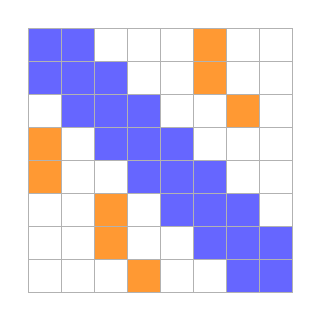
\begin{tikzpicture}[scale=0.42]
        \foreach \i in {0,...,7} {
          \foreach \j in {0,...,7} {
            \pgfmathtruncatemacro{\d}{abs(\i-\j)}
            \ifnum\d<2
              \fill[blue!60] (\i,-\j) rectangle ++(1,-1);
            \fi
          }
        }
        \foreach \i/\j in {0/5, 1/5, 2/6, 3/0, 4/0, 5/2, 6/2, 7/3} {
          \fill[orange!80] (\j,-\i) rectangle ++(1,-1);
        }
        \draw[step=1, gray!60, thin] (0,-8) grid (8,0);
      \end{tikzpicture}

      {\footnotesize Blue: local window. Orange: selected blocks.}
    \end{column}
  \end{columns}
\end{frame}

\section{Results}

\begin{frame}{ROUGE-L on three benchmarks}
  \centering
  \begin{tabular}{lccc}
    \toprule
    Model & arXiv & PubMed & GovReport \\
    \midrule
    BART (1{,}024 tokens) & 39.8 & 40.1 & 50.2 \\
    Longformer & 41.2 & 41.6 & 52.4 \\
    BigBird & 41.3 & 41.8 & 52.7 \\
    Ours & \textbf{41.6} & \textbf{42.3} & \textbf{53.4} \\
    \bottomrule
  \end{tabular}

  \vspace{1em}
  Peak memory at 4{,}096 tokens: 23\,GB, against 38\,GB for full attention.
\end{frame}

\begin{frame}{Next steps}
  \begin{itemize}
    \item Ablate the block size $b$ and the number of selected blocks $r$.
    \item Human evaluation of factual consistency on 100 arXiv summaries.
    \item Camera-ready deadline: 4 December.
  \end{itemize}
\end{frame}

\end{document}
